% CVPR 2022 Paper Template
% based on the CVPR template provided by Ming-Ming Cheng (https://github.com/MCG-NKU/CVPR_Template)
% modified and extended by Stefan Roth (stefan.roth@NOSPAMtu-darmstadt.de)

\documentclass[10pt,twocolumn,letterpaper,pagenumbers]{article}

% Page geometry
\usepackage[
    letterpaper,
    textwidth=6.875in,      
    textheight=8.875in,     
    columnsep=0.3125in,     
    top=1in,                
    bottom=1.125in,         
    left=0.8125in,          
    right=0.8125in          
]{geometry}

%%%%%%%%% PAPER TYPE  - PLEASE UPDATE FOR FINAL VERSION
\usepackage[review]{cvpr}      % To produce the REVIEW version
%\usepackage{cvpr}              % To produce the CAMERA-READY version
%\usepackage[pagenumbers]{cvpr} % To force page numbers, e.g. for an arXiv version

\setlength{\parindent}{1pc}  % 1 pica indent
\setlength{\parskip}{0pt}     % No space between paragraphs

\usepackage{caption}
\captionsetup{
  font=small,
  labelfont=bf,
  justification=centering
}

% Include other packages here, before hyperref.
\usepackage{graphicx}
\usepackage{amsmath}
\usepackage{amssymb}
\usepackage{booktabs}


% It is strongly recommended to use hyperref, especially for the review version.
% hyperref with option pagebackref eases the reviewers' job.
% Please disable hyperref *only* if you encounter grave issues, e.g. with the
% file validation for the camera-ready version.
%
% If you comment hyperref and then uncomment it, you should delete
% ReviewTempalte.aux before re-running LaTeX.
% (Or just hit 'q' on the first LaTeX run, let it finish, and you
%  should be clear).
\usepackage[pagebackref,breaklinks,colorlinks]{hyperref}


% Support for easy cross-referencing
\usepackage[capitalize]{cleveref}
\usepackage{float}
\crefname{section}{Sec.}{Secs.}
\Crefname{section}{Section}{Sections}
\Crefname{table}{Table}{Tables}
\crefname{table}{Tab.}{Tabs.}


%%%%%%%%% PAPER ID  - PLEASE UPDATE
\def\cvprPaperID{} % *** Enter the CVPR Paper ID here
\def\confName{}
\def\confYear{2022}



\begin{document}
\pagestyle{plain} %To force page numbers

%%%%%%%%% TITLE - PLEASE UPDATE
\title{CNN-Based Malaria Parasite Recognition in Human Blood Smear Images}


\maketitle


%%%%%%%%% BODY TEXT
\section{Problem statement and application} Malaria diagnosis relies on manual blood smear analysis, a process that is time consuming, expertise dependent, and prone to human error, particularly in resource-limited settings. While convolutional neural networks (CNNs) have been applied to automate malaria parasite detection ~\cite{JMAMSJ}, challenges remain due to high visual similarity between parasite stages, staining variability, mislabeling and changes in smear quality which causes errors and inconsistencies in the data ~\cite{ahamed_malaria_2025}, ~\cite{rubio_maturana_2022}.This project aims to evaluate CNN architectures across malaria datasets, addressing labeling and smear variability challenges, compare training strategies, and identify robust models.

\section{Image dataset selection}
To study how CNN models perform on datasets of different difficulty levels, three publicly available malaria microscopy datasets are used: the Malaria Dataset ~\cite{miracle9to9}, P. vivax Malaria Infected Human Blood Smears ~\cite{orvile}, and Malaria Plasmodium Vivax Specie ~\cite{saife245}. These datasets differ in the number of classes, image quality, and visual complexity, enabling comparison across binary, multi-class, and fine-grained classification tasks. A summary of the datasets is provided in Table~\ref{tab:datasets}, with example images from each dataset shown below.

\begin{table}[H]
\centering
\caption{Summary of malaria microscopy datasets used in this project.}
\label{tab:datasets}
\resizebox{\linewidth}{!}{
\begin{tabular}{lcccc}
\toprule
Dataset & Classes & Images & Image Size & Format \\
\midrule
miracle9to9 & 2 & 27,558 & $128 \times 128$ & PNG \\
orvile & 4 (parasite stages) & 1,328 & Variable & JPEG \\
saife245 & Multiple (fine-grained) & 1,364 & Variable & JPEG/PNG \\
\bottomrule
\end{tabular}
}
\end{table}
\begin{figure}[H]
  \centering
  
\includegraphics[width=0.2\linewidth]{cvpr2022-author_kit-v1_1-1-2/latex/Parasitised.png}
  \caption{Example microscopy image from  P. vivax malaria infected human blood smear(orvile.)}
  \label{fig:orvile_example}
\end{figure}

\begin{figure}[H]
  \centering
  
\includegraphics[width=0.2\linewidth]{cvpr2022-author_kit-v1_1-1-2/latex/0b04ec46-5119-4cda-8c35-c4e5b6f0eed0.png}
  \caption{Example microscopy image from Malaria plasmodium vivax specie (saife245.)}
  \label{fig:saife245_example}
\end{figure}

\begin{figure}[H]
  \centering
  
\includegraphics[width=0.2\linewidth]{cvpr2022-author_kit-v1_1-1-2/latex/003a89b0-a095-417a-8dd6-f408339bbc68.png}
  \caption{Example microscopy image from the Malaria Dataset (miracle9to9).}
  \label{fig:miracle9to9}
\end{figure}

\section{Methodology}
This project evaluates three CNN architectures ResNet-18~\cite{resnet}, VGG-16~\cite{vgg}, and MobileNet-V2~\cite{mobilenet} trained on malaria datasets of varying complexity~\cite{JMAMSJ}. Prior to training, a rigorous preprocessing pipeline ensures data consistency: all images are resized to a standardized resolution, normalized to account for staining variability, and augmented via rotations and flips to improve generalization~\cite{ahamed_malaria_2025}. The training will occur on the Google Colab cloud infrastructure with NVIDIA T4 GPUs to efficiently manage 11 distinct model cycles.
The experimental design involves nine models trained from scratch to compare performance across the binary, multi-class, and fine-grained datasets summarized in Table~\ref{tab:datasets}. Two additional models utilize transfer learning on complex sets like saife245~\cite{saife245}. Transfer learning is applied here because pre-trained weights leverage learned feature representations, which is essential when handling limited medical samples with high visual similarity~\cite{rubio_maturana_2022}. Architectures are compared using Accuracy, Precision, Recall, and F1-score to handle class imbalances and prioritize the minimization of false negatives. Finally, Grad-CAM~\cite{gradcam} visualizations will verify that the CNNs identify parasitic chromatin rather than staining artifacts, providing a qualitative layer to the quantitative performance analysis~\cite{ahamed_malaria_2025}.

\onecolumn



\section{Gantt chart ~\cite{gantt_chart}}
\begin{figure}[H]
  \centering
  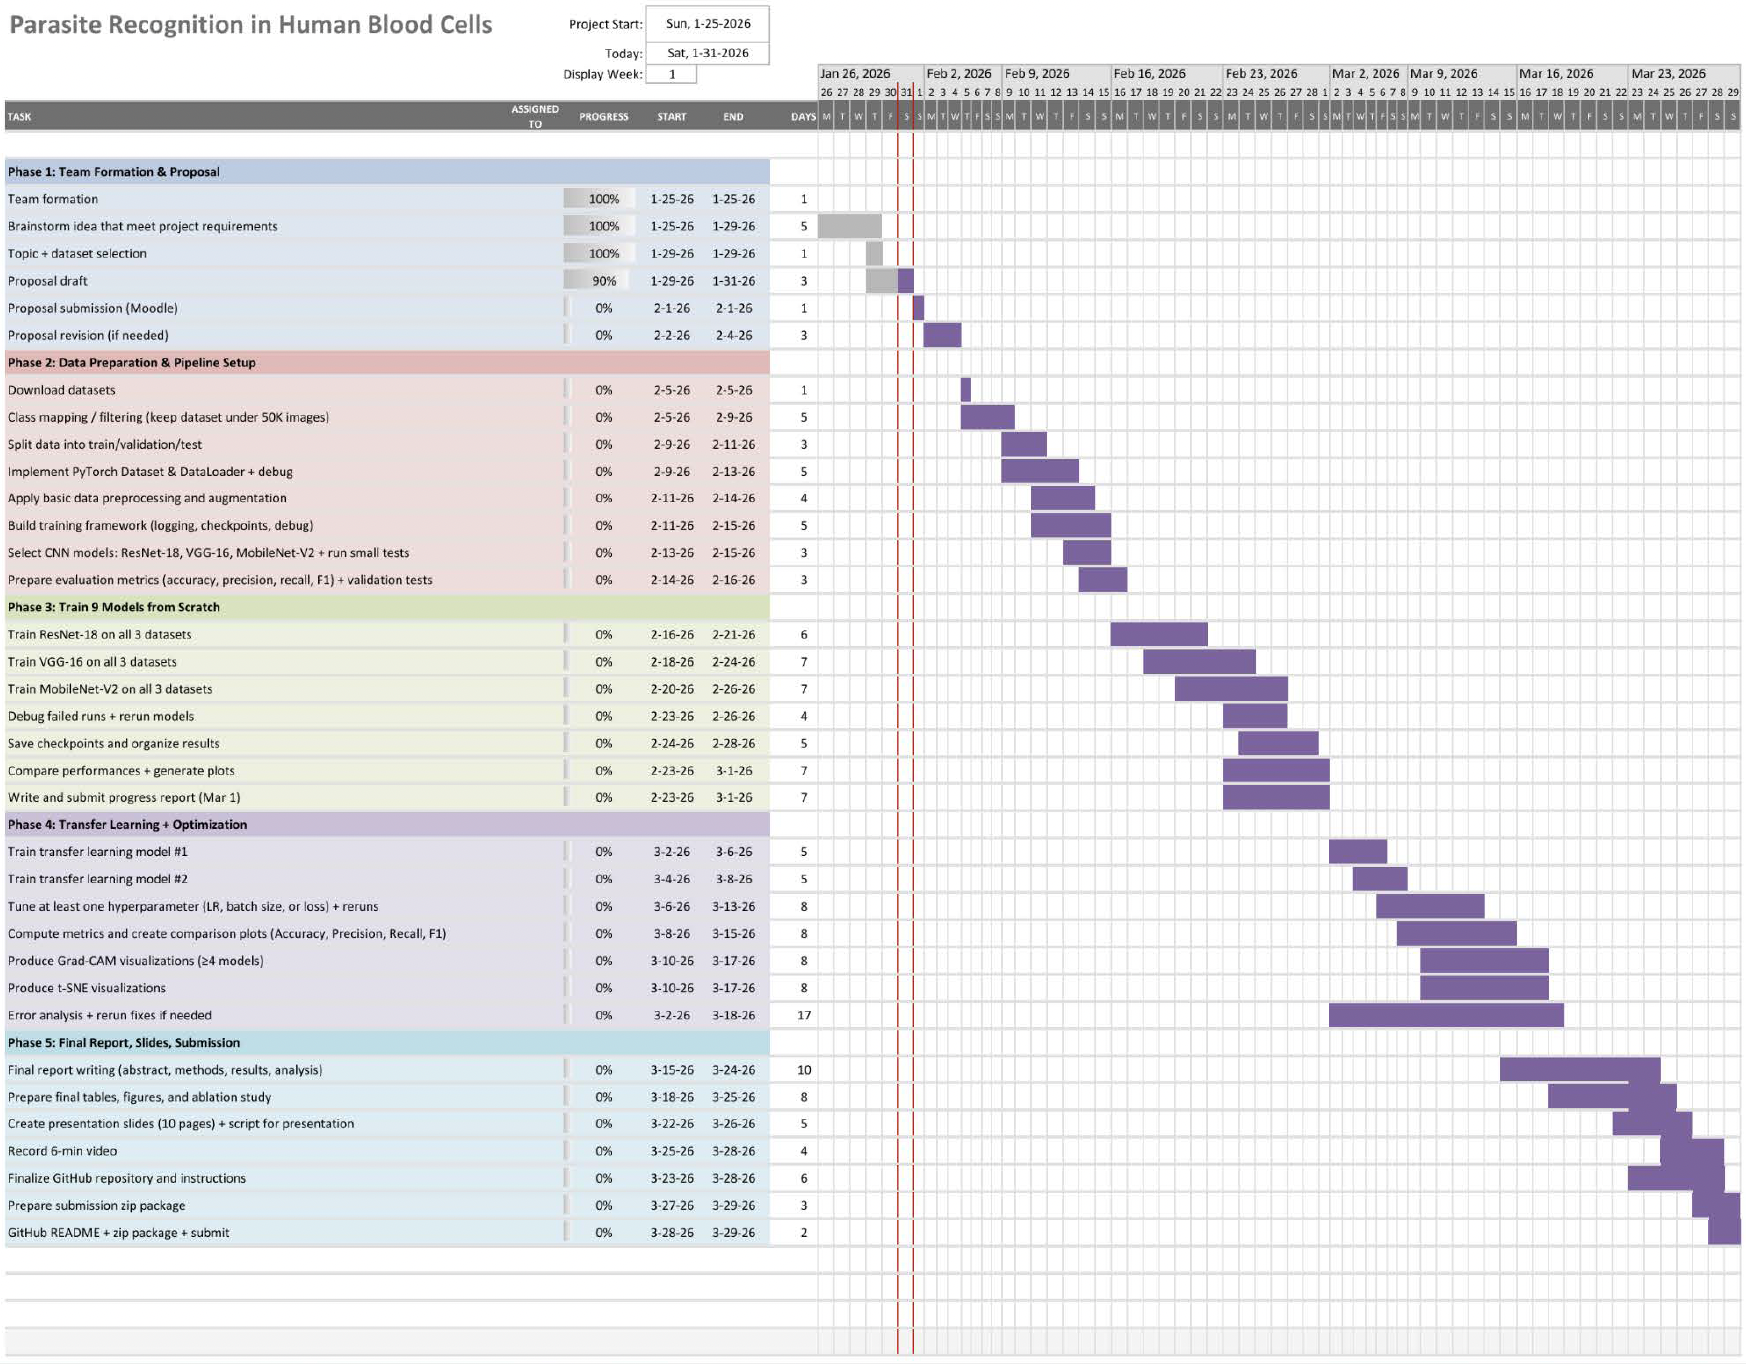
\includegraphics[width=0.9\linewidth]{gantt.png}
  \caption{Gantt chart illustrating the project timeline, milestones, and deliverables.}
  \label{fig:gantt}
\end{figure}
\twocolumn

\section{Bibliography}


%%%%%%%%% REFERENCES
{\small
\bibliographystyle{ieee_fullname}
\bibliography{egbib}
}

\end{document}
